\documentclass[10pt,twocolumn,letterpaper]{article}

\usepackage{cvpr}
\usepackage{times}
\usepackage{epsfig}
\usepackage{graphicx}
\usepackage{amsmath}
\usepackage{amssymb}

\usepackage{subcaption}
\usepackage{multirow}

% Include other packages here, before hyperref.

% If you comment hyperref and then uncomment it, you should delete
% egpaper.aux before re-running latex.  (Or just hit 'q' on the first latex
% run, let it finish, and you should be clear).
\usepackage[breaklinks=true,bookmarks=false]{hyperref}

\def\cvprPaperID{****} % *** Enter the CVPR Paper ID here
\def\httilde{\mbox{\tt\raisebox{-.5ex}{\symbol{126}}}}

% Pages are numbered in submission mode, and unnumbered in camera-ready
%\ifcvprfinal\pagestyle{empty}\fi
\setcounter{page}{1}
\begin{document}

%%%%%%%%% TITLE
\title{MLCV Coursework 1 Report}

\author{Shinyoung Yu\\
20200405\\
School of Computing\\
{\tt\small sahaa0918@kaist.ac.kr}
% For a paper whose authors are all at the same institution,
% omit the following lines up until the closing ``}''.
% Additional authors and addresses can be added with ``\and'',
% just like the second author.
% To save space, use either the email address or home page, not both
\and
Jiyun Park\\
20210263\\
School of Computing\\
{\tt\small jiyun02@kaist.ac.kr}
}

\maketitle
%\thispagestyle{empty}

% \begin{abstract}
The ABSTRACT is to be in fully justified italicized text, at the top of the left-hand column, below the author and affiliation information.
Use the word ``Abstract'' as the title, in 12-point Times, boldface type, centered relative to the column, initially capitalized.
The abstract is to be in 10-point, single-spaced type.
Leave two blank lines after the Abstract, then begin the main text.
Look at previous \confName abstracts to get a feel for style and length.
\end{abstract}   
\section{Eigenfaces}
\label{sec:intro}

Face data is the base dataset for our experiment. This consists of 520 data with 52 classes and 10 data for each class. We will conduct the upcoming experiments by dividing the data for each class into an 8:2 train-test split.

%-------------------------------------------------------------------------
\subsection{Eigenfaces}

There are two method to conduct PCA: PCA($S=AA^T$) and low dimensional PCA($S=A^TA$). We compare two methods on training dataset with size 2576*416(D*N).

\begin{figure}[htbp]
	\centering
	\begin{subfigure}[t]{0.48\linewidth}
		\centering
		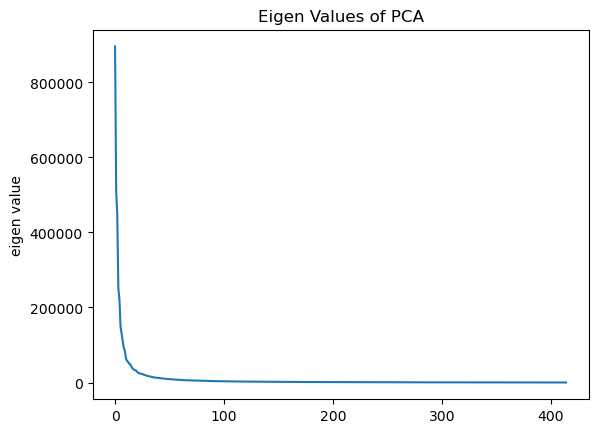
\includegraphics[width=\linewidth]{image/q1_eigval_pca.png}
		\caption{nonzero eigenvalues of PCA}
		\label{fig:eigval_pca}
	\end{subfigure}%
	\hfill
	\begin{subfigure}[t]{0.48\linewidth}
		\centering
		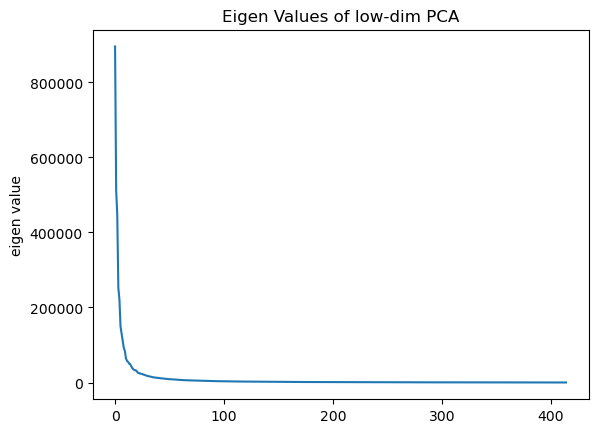
\includegraphics[width=\linewidth]{image/q1_eigval_lowdim.png}
		\caption{nonzero eigenvalues of low-dimensional PCA}
		\label{fig:eigval_lowdim}
	\end{subfigure}
	\caption{Comparison between eigenvalues of PCA methods}
	\label{fig:q1_eigval}
\end{figure}

As shown in \cref{fig:q1_eigval} both methods have the same nonzero eigenvalues. Specifically, PCA has 2576 nonzero eigenvalues, and low-dimensional PCA has 416. However, when selecting values bigger than $\frac{1}{100}$, both methods yield 415 eigenvalues. This is because, given matrix sizes of 2576x2576 and 416x416, the maximum ranks are 2576 and 416, respectively. But since we have 416 data points, the PCA projection subspace can at most capture 415 meaningful dimensions, resulting in 415 eigenvalues larger than $\frac{1}{100}$. From this comparison (\cref{fig:q1_eigval}), we conclude that both methods yield the same eigenvalues, and their top 415 eigenvectors are also identical.

The only difference between them is computation time: PCA takes 8.015s, while low-dimensional PCA takes 1.092s. Low-dimensional PCA is faster because, in our case, the data dimension exceeds the number of data points, making its covariance matrix smaller than that of PCA. Based on this time efficiency, we use low-dimensional PCA going forward. % 시간복잡도는 O(N^3)인데 이것보단 적게 차이나는데 어쩌지!!


\subsection{Image reconstuction using Eigenfaces}
Using pca basis from above, we perform face reconstruction. \cref{fig:recon_train} and \cref{fig:recon_test} shows reconstruction results using different numbers of PCA bases. As seen in the images, the reconstruction become more accurate with more bases. When using only 10 bases, the results resemble the mean face(\cref{fig:q1_meanface}) of training data. This occurs because the PCA basis is oriented to capture common features by maximizing data variance. Thus, with a small number of bases, the reconstruction reflects common features of the dataset more strongly than specific details of each image.

\begin{figure}
	\centering
	\begin{subfigure}[t]{0.2\linewidth}
		\centering
		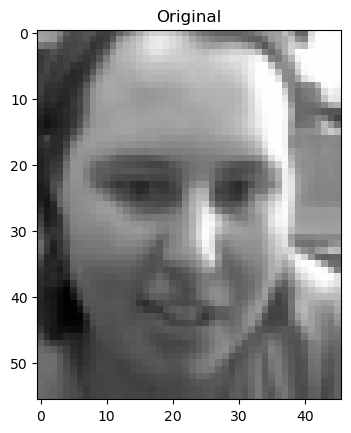
\includegraphics[width=\linewidth]{image/q1_recon_train_original.png}
		\caption{original}
		\label{fig:train_re_original}
	\end{subfigure}%
	\hfill
	\begin{subfigure}[t]{0.2\linewidth}
		\centering
		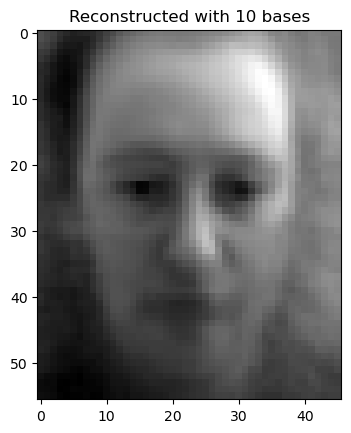
\includegraphics[width=\linewidth]{image/q1_recon_train_10.png}
		\caption{10 bases}
		\label{fig:train_re_10}
	\end{subfigure}
    \hfill
	\begin{subfigure}[t]{0.2\linewidth}
		\centering
		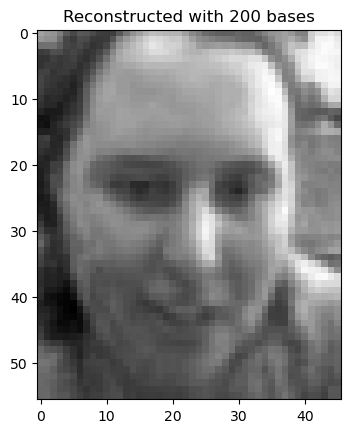
\includegraphics[width=\linewidth]{image/q1_recon_train_200.png}
		\caption{200 bases}
		\label{fig:train_re_200}
	\end{subfigure}
    \hfill
	\begin{subfigure}[t]{0.2\linewidth}
		\centering
		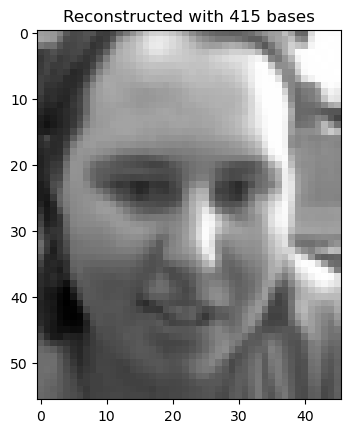
\includegraphics[width=\linewidth]{image/q1_recon_train_415.png}
		\caption{415 bases}
		\label{fig:train_re_415}
	\end{subfigure}
	\caption{Training data reconstruction results}
	\label{fig:recon_train}
\end{figure}

\begin{figure}
	\centering
	\begin{subfigure}[t]{0.2\linewidth}
		\centering
		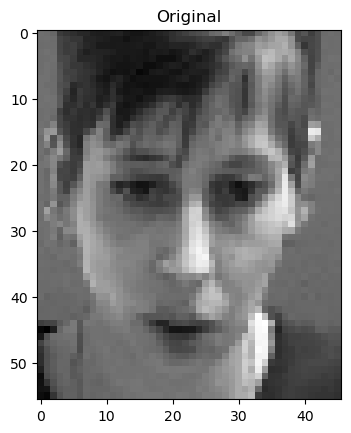
\includegraphics[width=\linewidth]{image/q1_recon_test_original.png}
		\caption{original}
		\label{fig:test_re_original}
	\end{subfigure}%
	\hfill
	\begin{subfigure}[t]{0.2\linewidth}
		\centering
		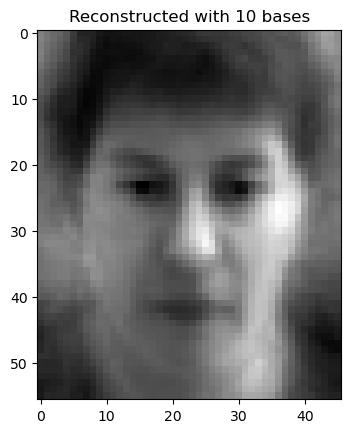
\includegraphics[width=\linewidth]{image/q1_recon_test_10.png}
		\caption{10 bases}
		\label{fig:test_re_10}
	\end{subfigure}
    \hfill
	\begin{subfigure}[t]{0.2\linewidth}
		\centering
		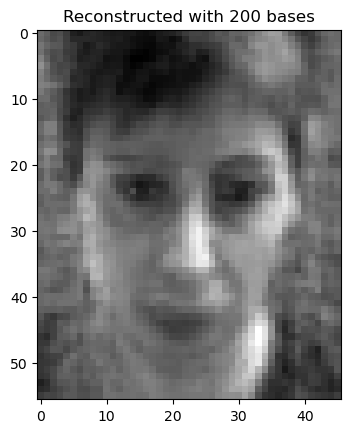
\includegraphics[width=\linewidth]{image/q1_recon_test_200.png}
		\caption{200 bases}
		\label{fig:test_re_200}
	\end{subfigure}
    \hfill
	\begin{subfigure}[t]{0.2\linewidth}
		\centering
		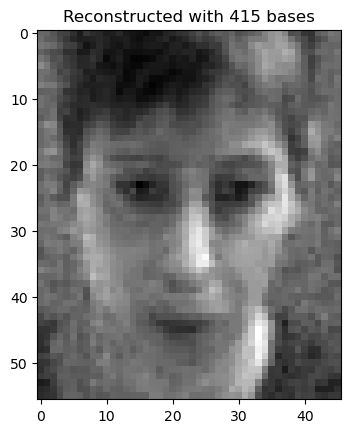
\includegraphics[width=\linewidth]{image/q1_recon_test_415.png}
		\caption{415 bases}
		\label{fig:test_re_415}
	\end{subfigure}
	\caption{Test data reconstruction results}
	\label{fig:recon_test}
\end{figure}

For more detailed analysis, we computed the reconstruction error. The theoretical error is given by $\sum_{i=n+1}^M \lambda_i$ where $n$is the number of bases we used for the reconstruction, $M$is total number of PCA bases, and $\lambda_i$ is eigenvalues of unused eigenvectors. The actual reconstruction error can be calculated using L2-norm of difference between the original and reconstructed data.

\begin{figure}
	\centering
	\begin{subfigure}[t]{0.48\linewidth}
		\centering
		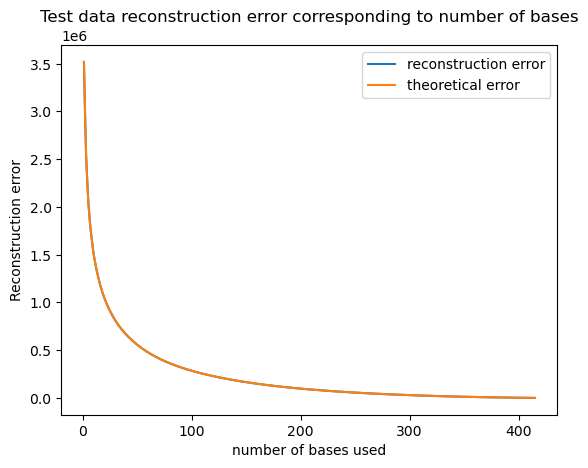
\includegraphics[width=\linewidth]{image/q1_recon_error_train.png}
		\caption{training data}
		\label{fig:recon_error_train}
	\end{subfigure}%
	\hfill
	\begin{subfigure}[t]{0.48\linewidth}
		\centering
		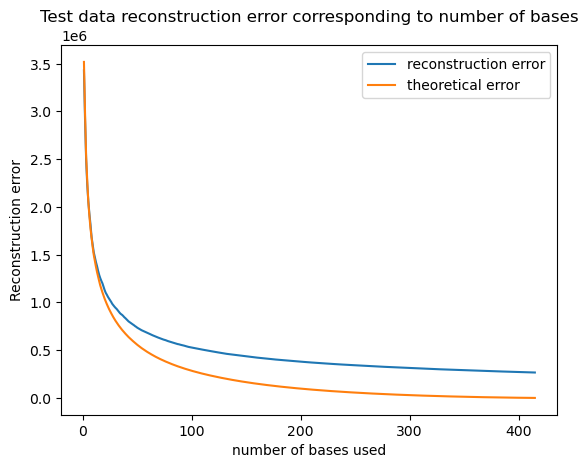
\includegraphics[width=\linewidth]{image/q1_recon_error_test.png}
		\caption{test data}
		\label{fig:recon_error_test}
	\end{subfigure}
	\caption{PCA reconstruction error}
	\label{fig:recon_error}
\end{figure}

As shown in \cref{fig:recon_error}, the reconstruction error from the training data matched the theoretical result. However, for the test data, while the graph’s shape was similar to the theoretical result, the actual values differed slightly. This may be because the PCA bases used for reconstruction were derived from the training data, not the test data.

\subsection{KNN classification using Eigenfaces}

We can also perform classification using PCA with NN classifier. As shown in \cref{fig:q1_knn_accuracy}, accuracy improves with more PCA bases and fewer neighbors($k$). More PCA bases preserve more data information, leading to accurate projections in the PCA subspace. For the number of neighbors, using fewer makes the classifier more sensitive to local information and better at preserving class boundaries, thus increasing classification accuracy.

In terms of time and memory, the number of neighbors made no significant difference. However, as shown in \cref{fig:q1_knn_time} and \cref{fig:q1_knn_memory}, the execution time and memory usage of the k-NN classifier linearly increase  with the number of PCA bases increase. This is because, the execution time and memory usage is $O(N\cdot M)$ where $N$ is the number of total data and $M$ is the number of PCA bases we used. Since $k$ only affects on final selection process, its impact during the computation is very small.

\begin{figure}
	\centering
	
	% 윗줄에 하나의 이미지, 크기는 0.48로 유지
	\begin{subfigure}[t]{0.48\linewidth}
		\centering
		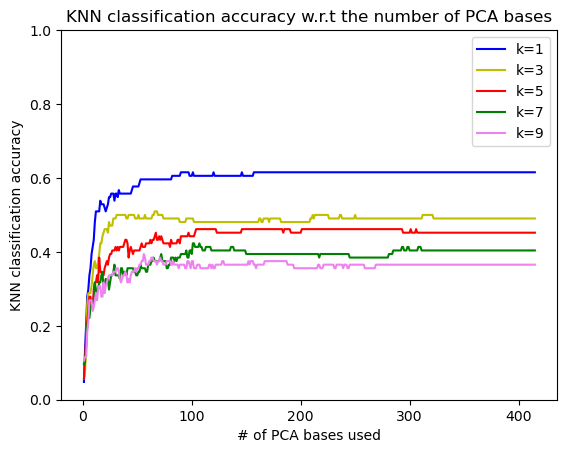
\includegraphics[width=\linewidth]{image/q1_accuracy.png}
		\caption{accuracy}
		\label{fig:q1_knn_accuracy}
	\end{subfigure}
	
    \vspace{0.5cm} % 이미지들 사이에 공간 추가

	% 아랫줄에 두 개의 이미지, 크기 동일하게 0.48
	\begin{subfigure}[t]{0.48\linewidth}
		\centering
		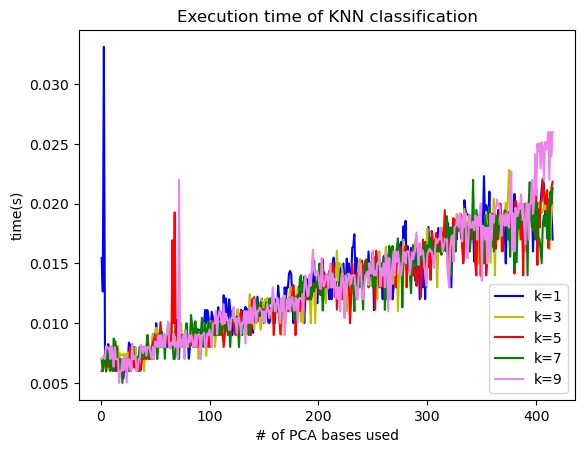
\includegraphics[width=\linewidth]{image/q1_time.png}
		\caption{running time}
		\label{fig:q1_knn_time}
	\end{subfigure}%
	\hfill
	\begin{subfigure}[t]{0.48\linewidth}
		\centering
		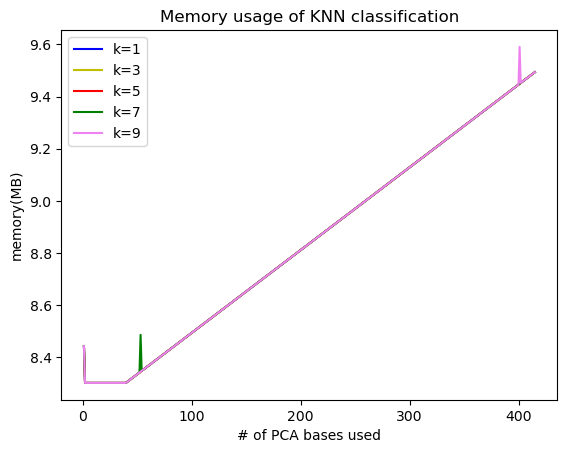
\includegraphics[width=\linewidth]{image/q1_memory.png}
		\caption{memory usage}
		\label{fig:q1_knn_memory}
	\end{subfigure}

	\caption{Analysis on KNN classification using PCA}
	\label{fig:pca_knn}
\end{figure}

However, its overall prediction accyracy is about 0.6, which is not that high. This might because, PCA is not very sophisticated model to capture all the detailed features of data. As we also check from the confusion matrix(\cref{fig:q1_cm}), there are many components outside the diagonal, that failed to be predicted.


Detailed prediction examples can be found in Appendix B, C.
\section{Incremental PCA}
\label{sec:intro}

%-------------------------------------------------------------------------
\subsection{Important parameter in implementation: $d_3$}
To implement incremental PCA, we utilized the algorithm from the "Online Learning" slides presented in class. Here, a key parameter is $d_2$ and $d_3$. When new data arrives in incremental PCA, computing the eigenspace model for this subset requires $O(\min(D, N')^3)$ time, where $N'$ is the number of data points in the subset. Additionally, merging this new eigenspace model with the existing data takes $O((d_1 + d_2 + 1)^3)$ time, where $d_1$ is equal to the previously computed eigenspace model's $d_3$ value. Therefore, to enhance time efficiency in incremental PCA, it is essential to keep $d_3$ small, although this results in a time-accuracy tradeoff by dropping less-significant eigenvector information, which is represented by our experiment result \cref{fig:q2-fig5}
\vspace{-0.5cm}

\begin{figure}[htbp]
	\centering
	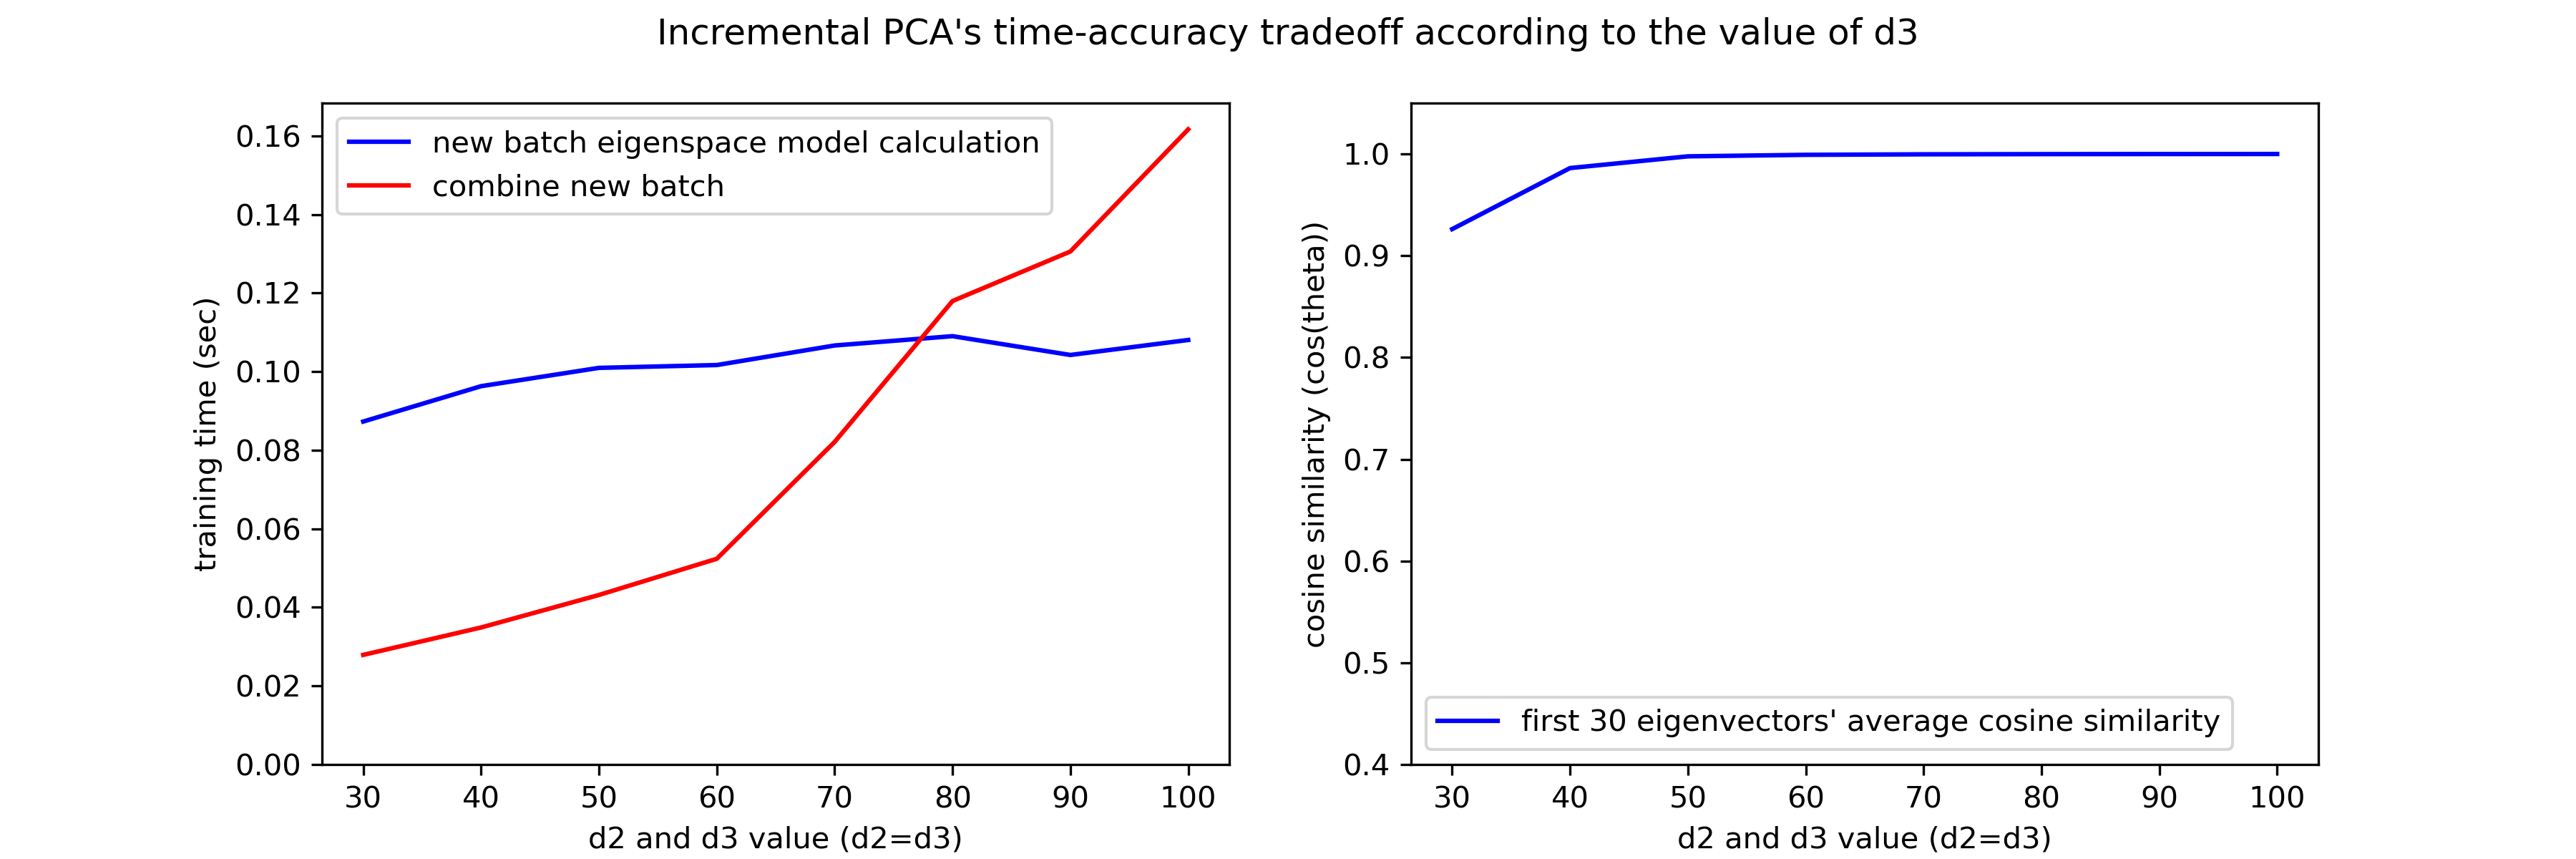
\includegraphics[width=\linewidth]{image/q2-fig5.png}
	
	\caption{Incremental PCA's time-accuracy tradeoff according to the value of $d_3$}
	\label{fig:q2-fig5}
\end{figure}
\vspace{-0.5cm}

\subsection{Comparison with other PCA}
We compared the results of each incremental PCA stage (i.e.adding training data in four batches) with the results of batch PCA in the following four aspects. In summary, incremental PCA is a good approximation of batch PCA, and even requires less training time.
\begin{itemize}
	\item Training time: For batch PCA, we measured training time by re-training the model each time new data was added. The results are shown in \cref{fig:q2-fig1}. Using one subset, the training time is approximately the same for both methods. However, as we add more data, the value of $N$ increases for batch PCA, while the values of $N'$ and $d_3$ remain constant for incremental PCA, maintaining constant time and improving time-wise efficiency.
	
	\item Accuracy of incremental PCA: In incremental PCA, time-accuracy tradeoff occurs since less-significant eigenvectors are dropped during $d_1 + d_2$ merging, retaining only the top $d_3$ eigenvectors. We calculated the cosine similarity of eigenvectors, eigenvalues, and mean vectors between incremental PCA at each stage and batch PCA calculated by corresponding data, as shown in \cref{fig:q2-fig2}. As more training data is added, the number of discarded less-significant eigenvectors increases, resulting in decreased similarity between eigenvectors; the similarity after adding the last subset is 0.856. For mean vectors and eigenvalues, cosine similarities are 1 and close to 1 respectively, indicating that the incremental PCA is a good approximation.
	
	\item Reconstruction error: Referring to \cref{fig:q2-fig3}, the reconstruction error for incremental PCA using all training data (i.e., after adding the 4th batch) is almost identical to that of batch PCA with the same amount of data. This also demonstrates that incremental PCA gives similar result to batch PCA.
	
	\item Face recognition accuracy: In the optimal settings of batch PCA found in Question1 (i.e. K=1 and bases=90) the accuracy ranks as follows: full-data batch PCA $>$ full-data incremental PCA $>$ PCA using only the first training set. This indicates that classification accuracy improves progressively with the increase in training data. Additionally, using incremental PCA in place of batch PCA results in an accuracy drop of approximately 6.67\%, also indicating a time-accuracy tradeoff.
	
\end{itemize}

\vspace{-0.5cm}
\begin{figure}[htbp]
	\centering
	\begin{subfigure}{0.48\linewidth}
		\centering
		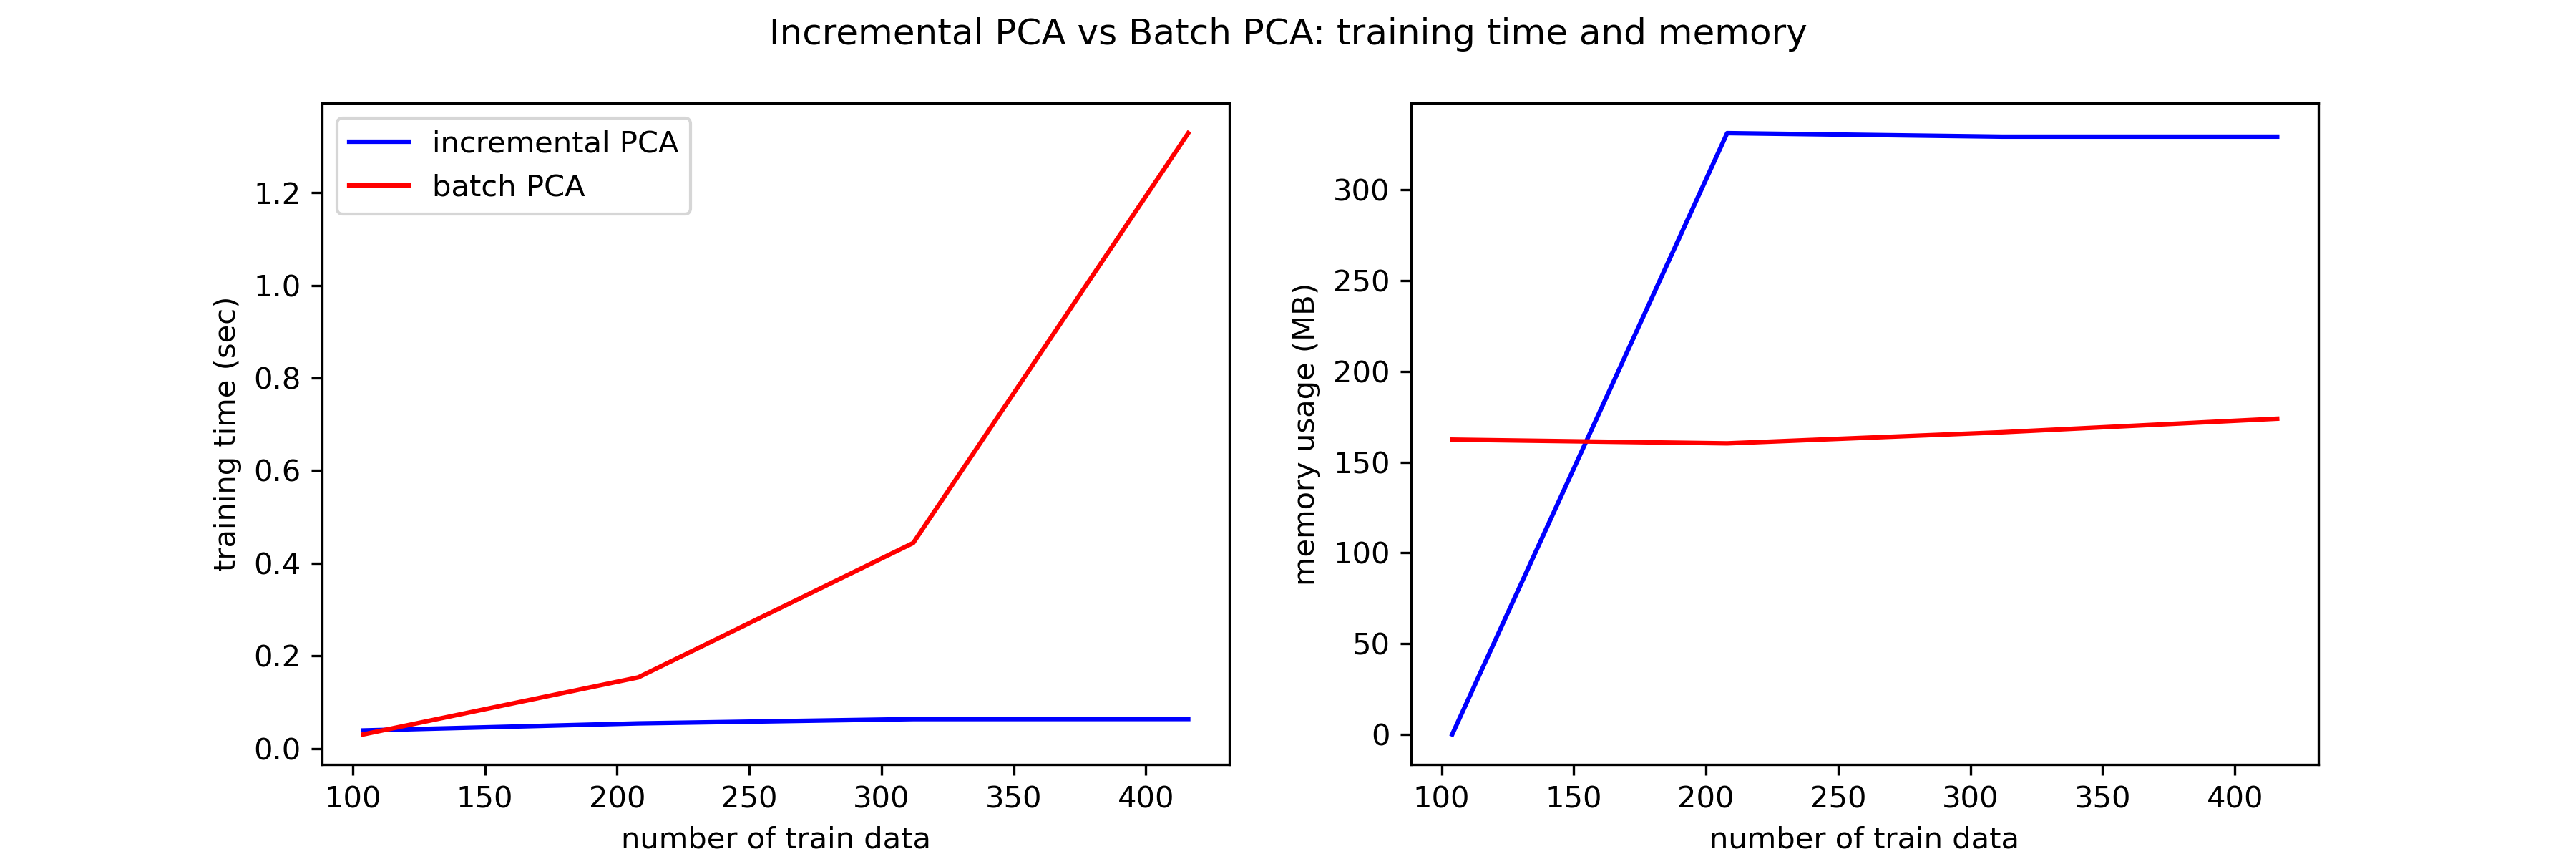
\includegraphics[width=\linewidth]{image/q2-fig1.png}
		\caption{Training time}
		\label{fig:q2-fig1}
	\end{subfigure}%
	\hfill
	\begin{subfigure}{0.48\linewidth}
		\centering
		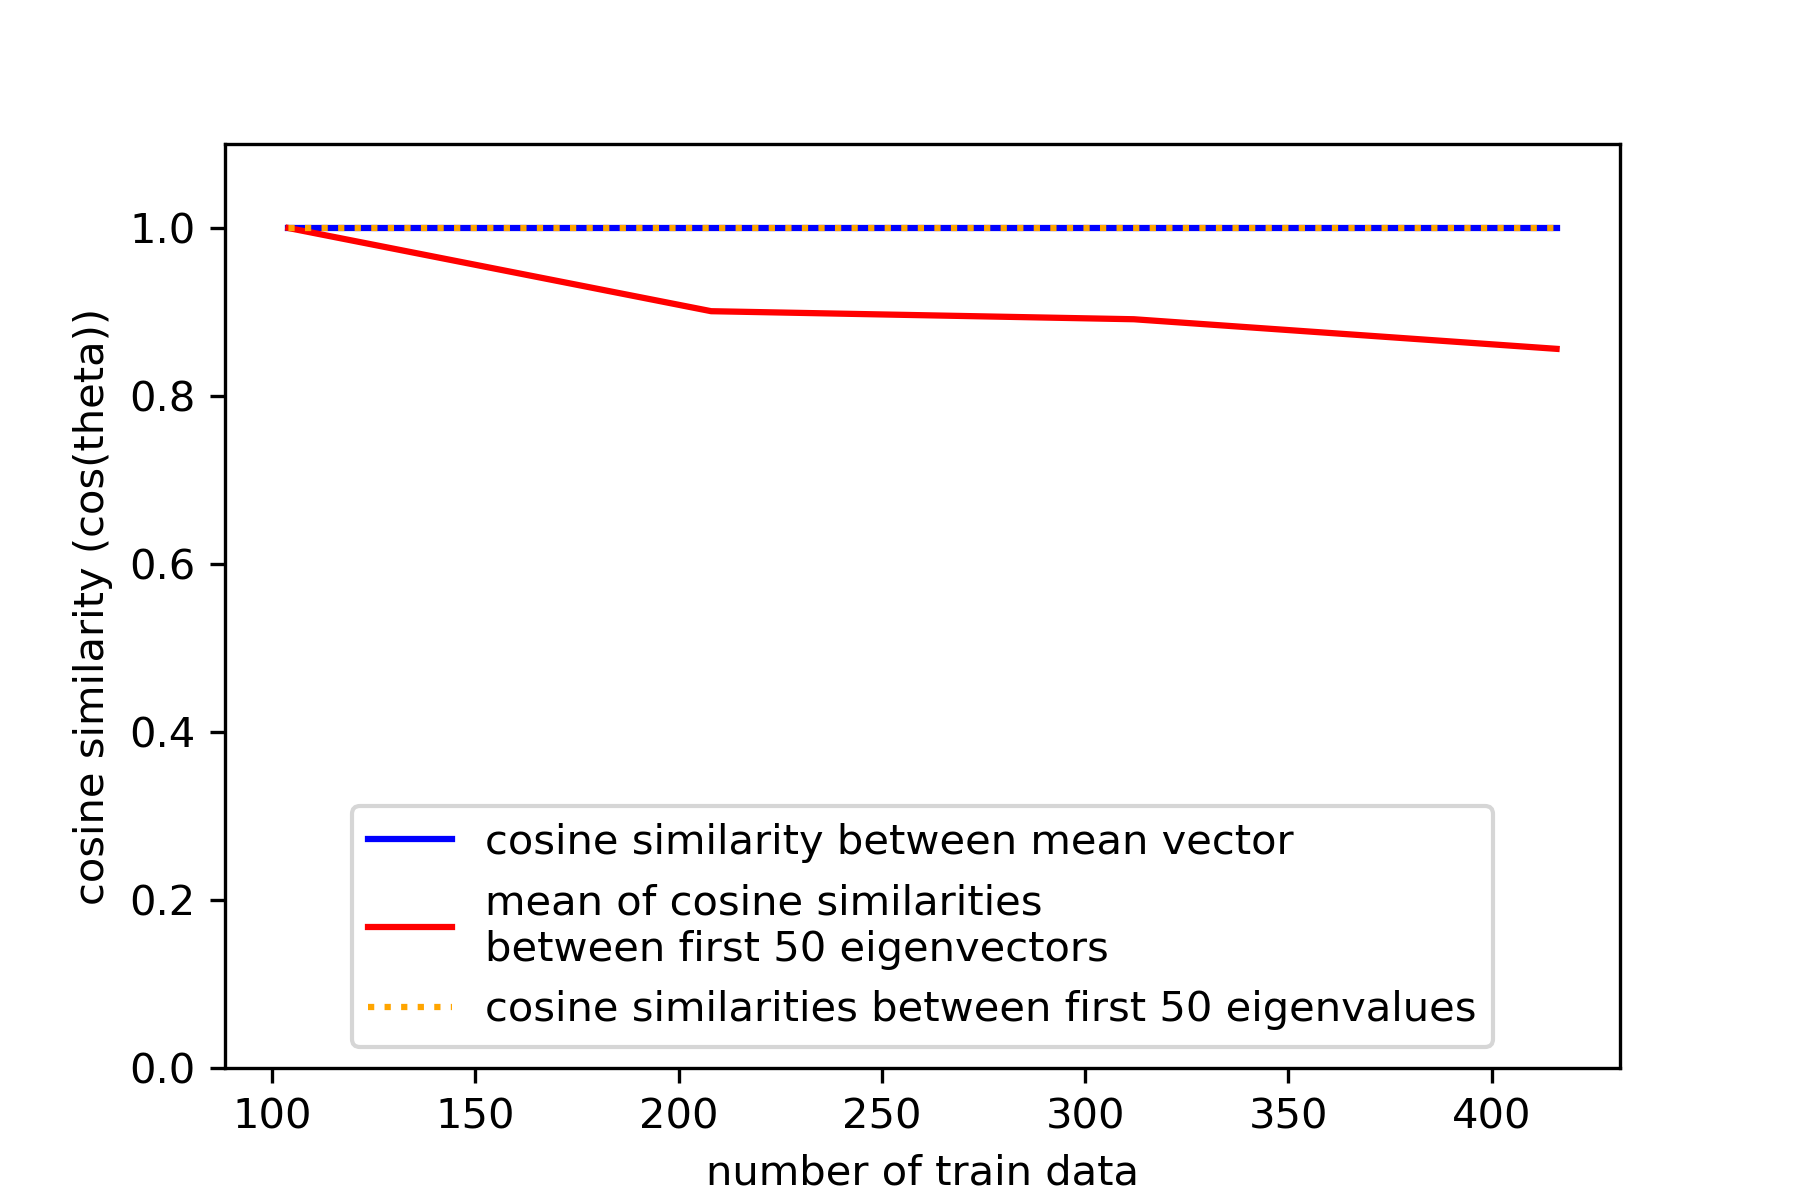
\includegraphics[width=\linewidth]{image/q2-fig2.png}
		\caption{Cosine similarity of results}
		\label{fig:q2-fig2}
	\end{subfigure}
	
	\begin{subfigure}{0.48\linewidth}
		\centering
		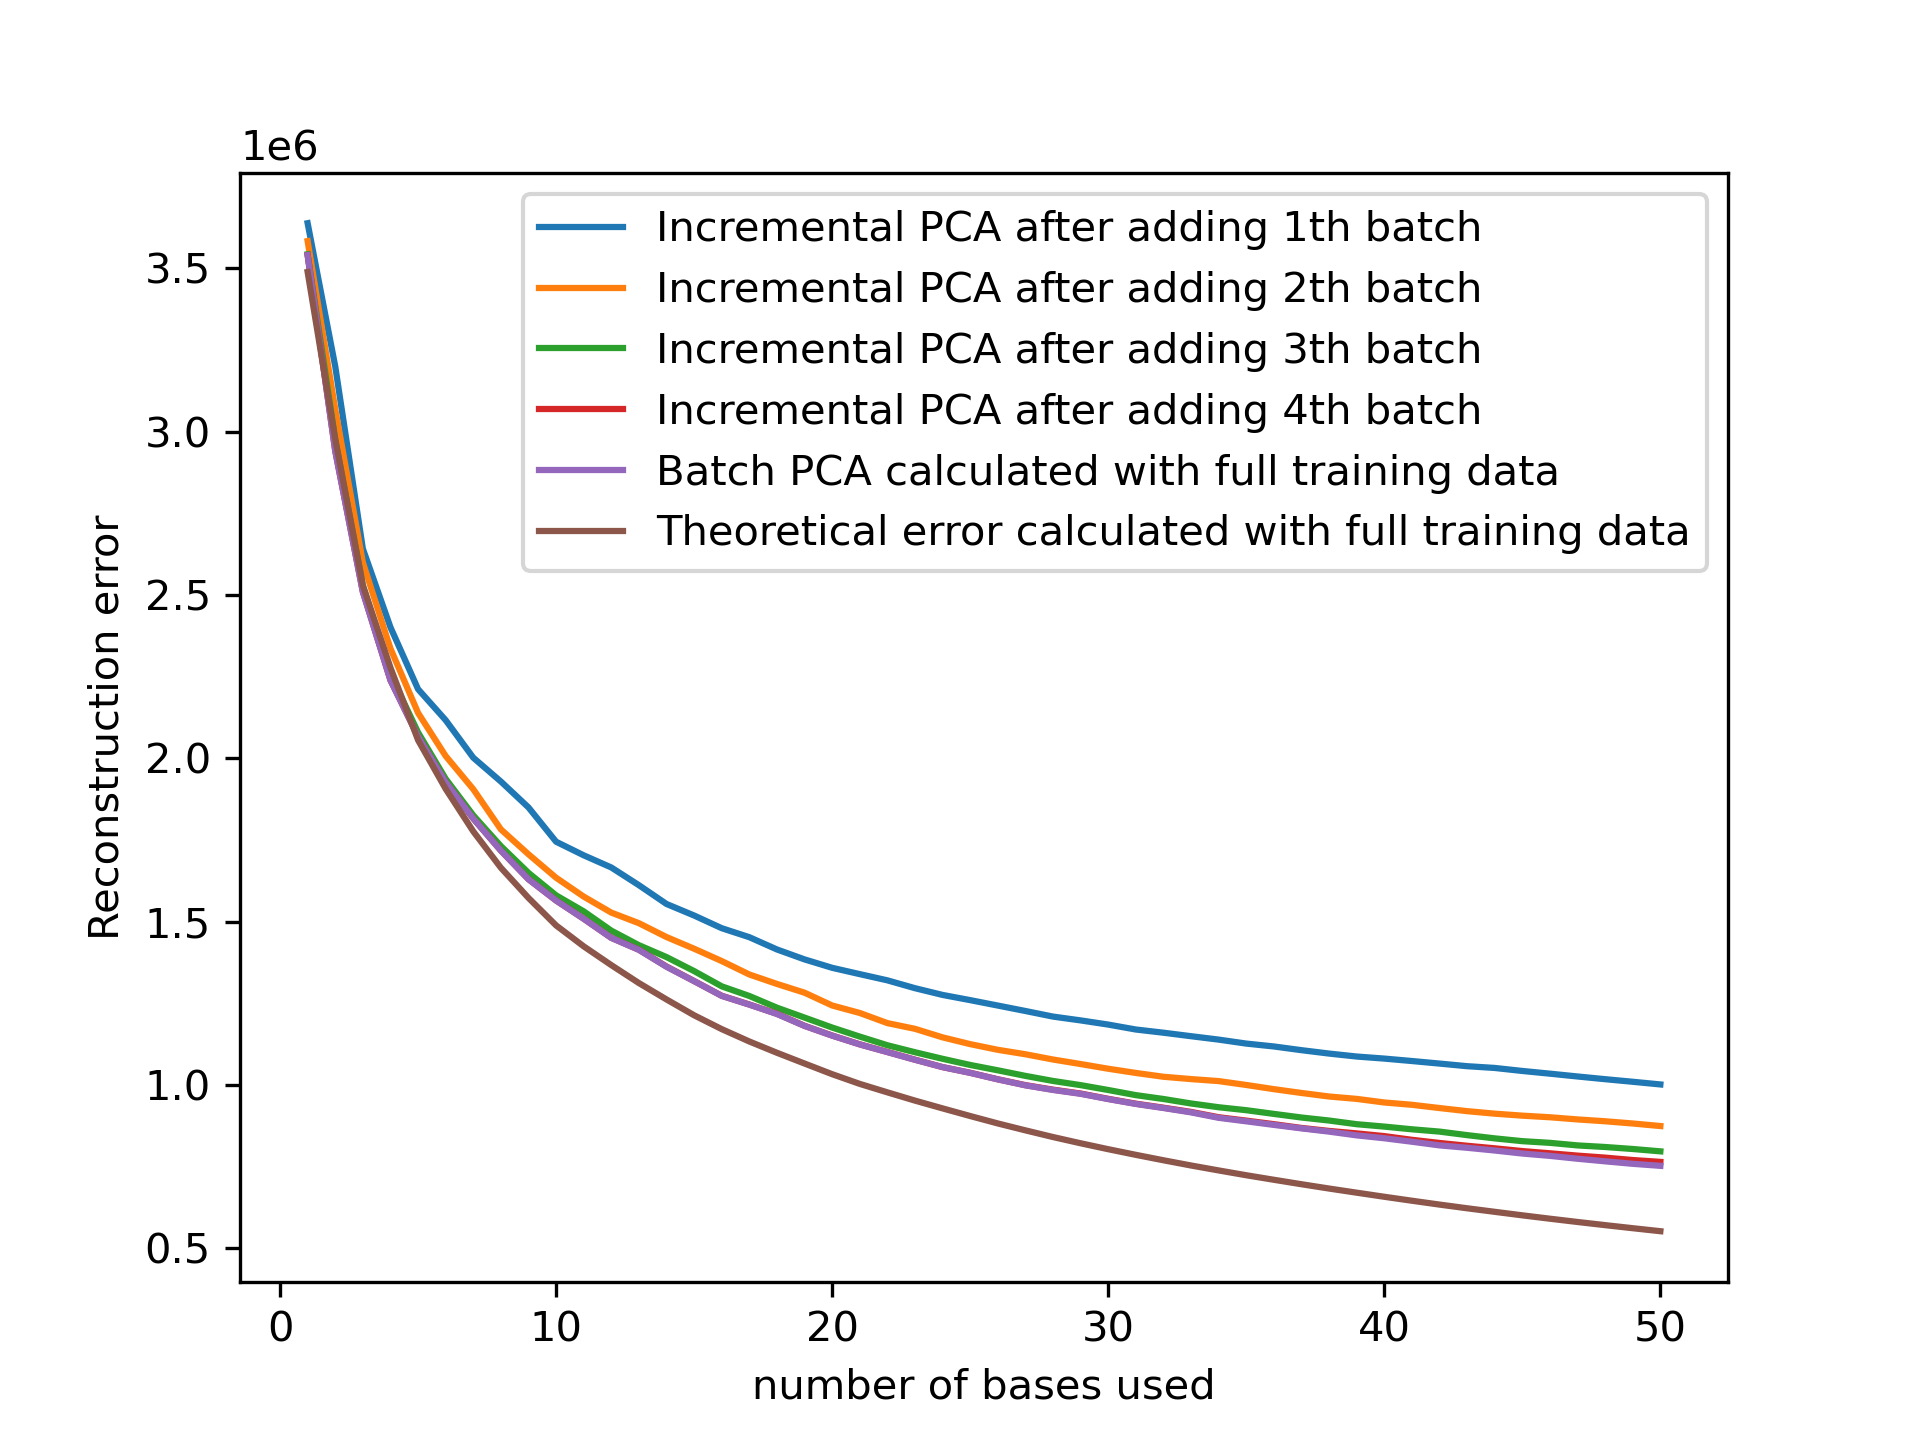
\includegraphics[width=\linewidth]{image/q2-fig3.png}
		\caption{Reconstruction error}
		\label{fig:q2-fig3}
	\end{subfigure}
	\hfill
	\begin{subfigure}{0.48\linewidth}
		\centering
		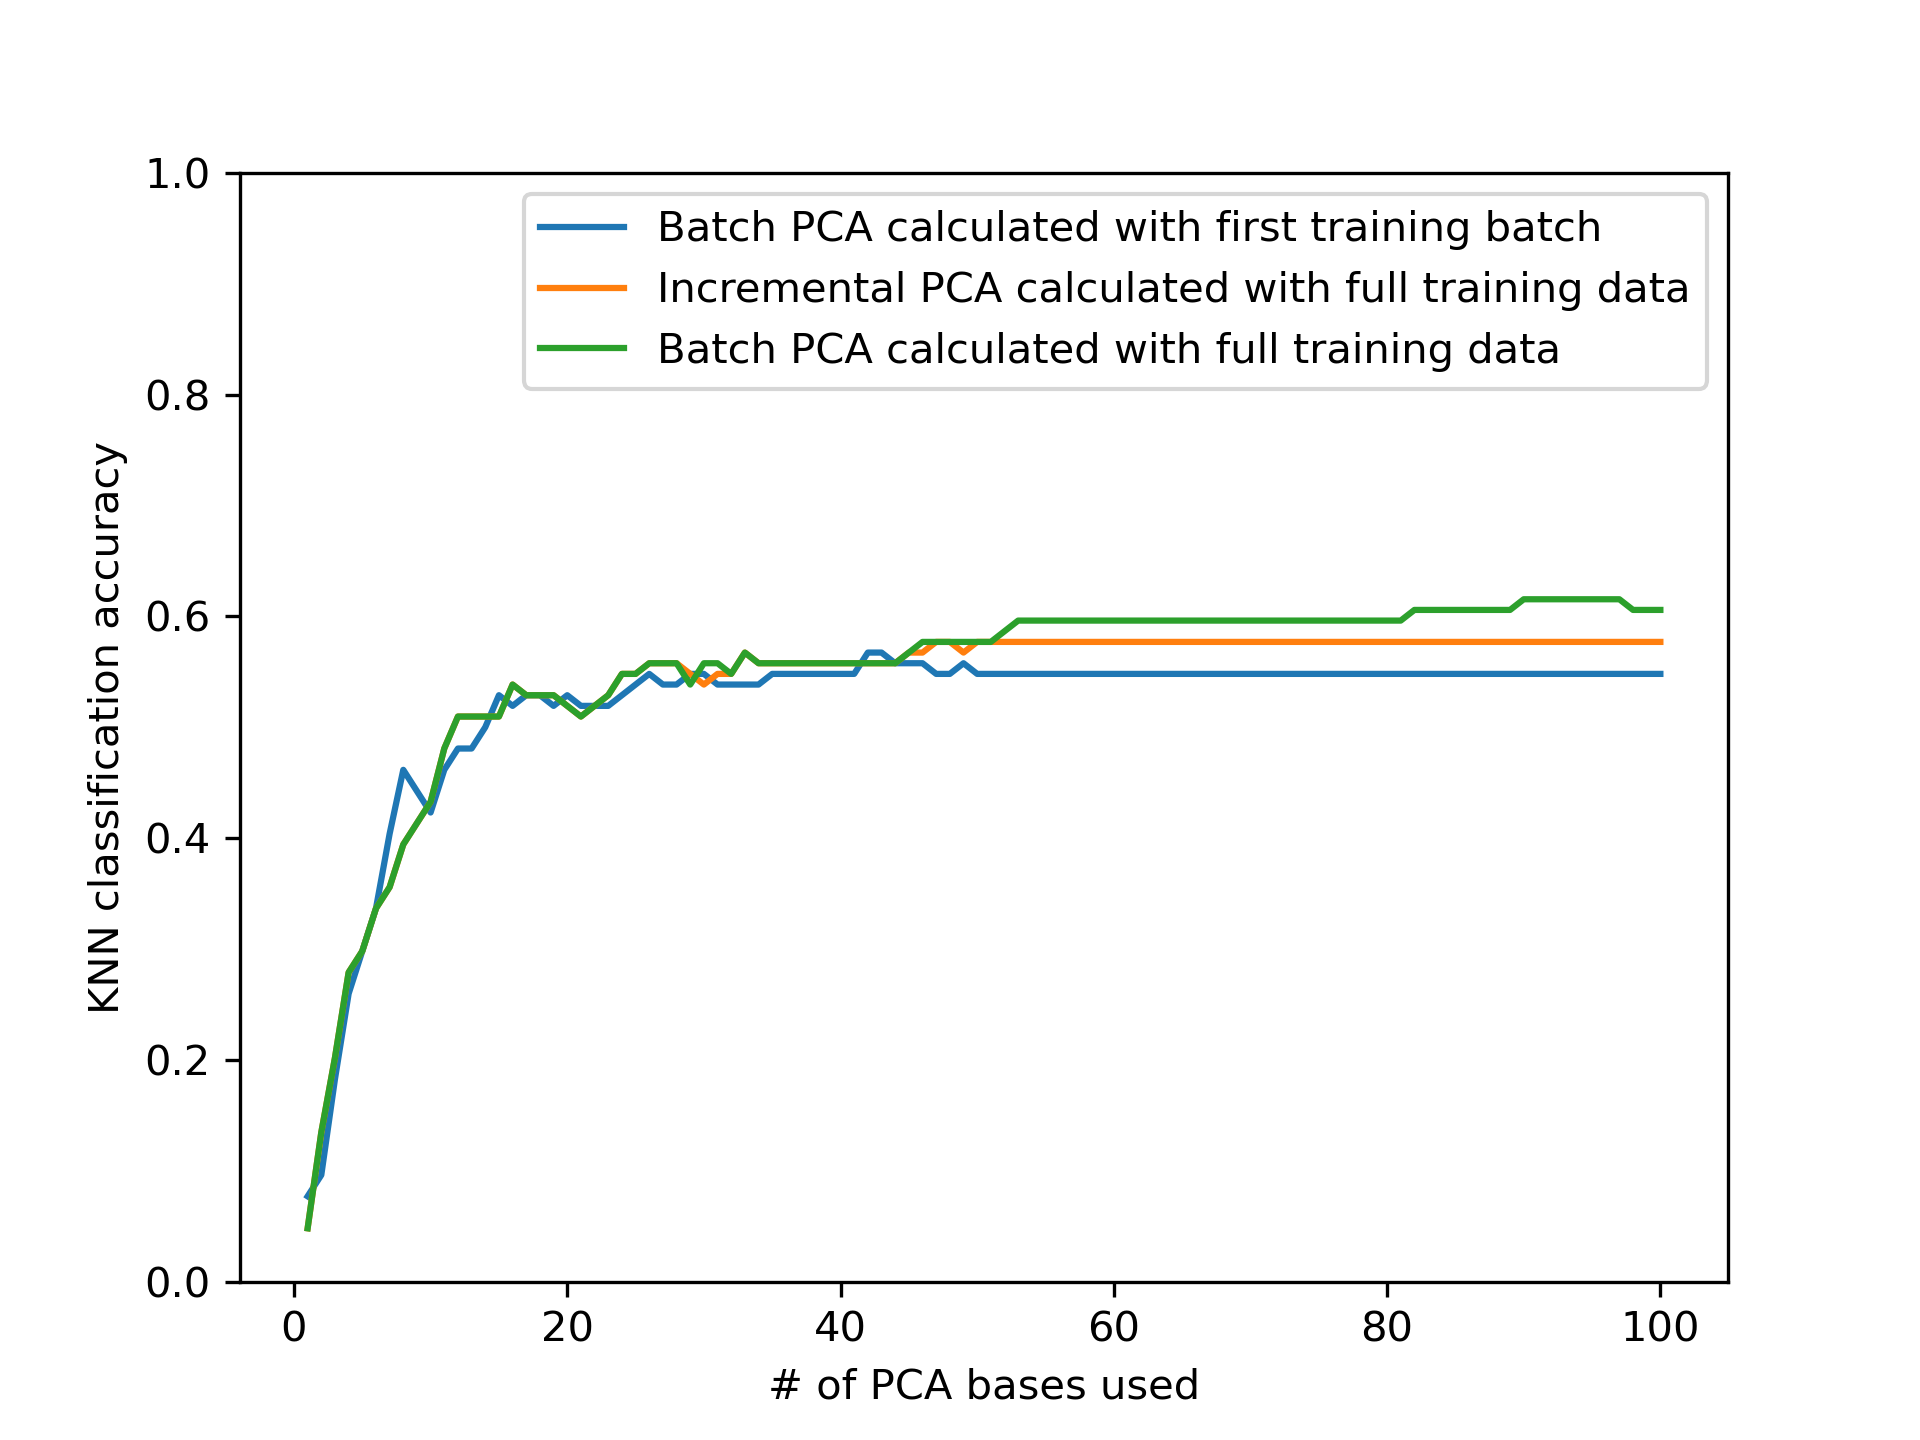
\includegraphics[width=\linewidth]{image/q2-fig4.png}
		\caption{NN-classification face recognition accuracy ($n\_nearest=1$)}
		\label{fig:q2-fig4}
	\end{subfigure}
	\caption{Comparison between Incremental and Batch PCA methods}
	\label{fig:q2}
\end{figure}
\vspace{-0.5cm}
\section{LDA Ensemble for Face Recognition}
\label{sec:intro}

PCA can effectively reduce the dimension of input data preserving important features. And LDA can maximize the variance of between-class while minimize between-class. Thus, using PCA-LDA is expected to increase computing efficiency and classification accuracy. In this section, we try to figure out the effect of PCA-LDA via some experiments.

%-------------------------------------------------------------------------
\subsection{Recognition accuracy of PCA-LDA}

To implement PCA-LDA, we set $M_{pca}$ and $M_{lda}$ by measuring classification accuracy with $M_{pca}$ from 1 to 415 and $M_{lda}$ from 1 to $min(M_{pca}-1, 51)$. This is because, the maximum possible projection dimension for PCA is $N-1$ since the total number of principal components can not be larger than overall data, and for LDA is $n_{class}-1$ since the number of direction for maximizing the distance of between-class and minimizing within-class cannot be larger than the total number of classes. As shown in \cref{fig:mpca_mlda}, accuracy peaked at $M_{pca}=150$ and $M_{lda}=50$. Higher $M_{lda}$ improves performance by enhancing data discrimination, while optimal $M_{pca}$ is between 100 and 200, balancing information retention and overfitting risk.


In LDA, the rank of within-class scatter matrix($S_w$) is $min(364, M_{pca})$, where $N-n_{class}=416-52=364$ and the rank of between-class scatter matrix($S_b$) is $n_{class}-1=51$. Since $\sum_{x\in D_i} (x-m_i) = 0$, each class is linearly dependent, so, $S_w = \sum_{i=1}^c \sum_{x\in D_i} (x-m_i)(x-m_i)^T$ has at most $N-n_{class}$ linearly independent row vectors. After reducing dimensions using PCA, the rank of $S_w$ cannot exceed $M_{pca}$ as the vectors are confined to the PCA subspace. For $S_b$ defined as $S_b = \sum_{i=1}^c (m_i-m)(m_i-m)^T$, it depends only ionly on class means, and since their relationship of class mean does not change after PCA projection since their relationships remain unchanged under PCA (a linear transformation), the maximum possible rank for $S_b$ is $N - n_{class}$.

Based on this observation, we decided to fix $M_{pca}=150$ and $M_{lda}=50$ for further experiments. 

\begin{figure}
  \centering
   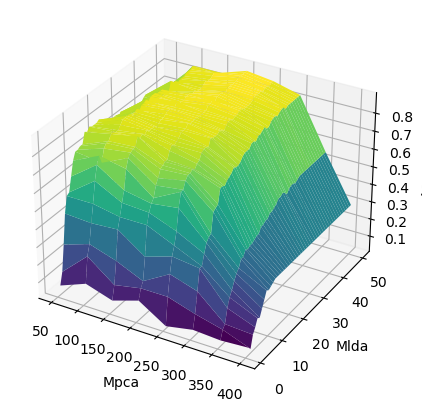
\includegraphics[width=0.8\linewidth]{image/mpca_mlda.png}

   \caption{Classification accuracy varying Mpca and Mlda}
   \label{fig:mpca_mlda}
\end{figure}


%-------------------------------------------------------------------------
\subsection{Result of PCA-LDA}

\cref{fig:q3_1_cm} is the confusion matrix of PCA-LDA classification result. As most of prediction result is on the diagonal entry, it indicates that most of prediction is successful. We take a closer look at success and failure cases. \cref{fig:q3_success} shows successfully predicted cases. Despite the different angles of the faces, the model infer the class accurately. \cref{fig:q3_fail} is failure cases. It seems that the prediction failed because of the similar glasses and face expression.


% %-------------------------------------------------------------------------
% \subsection{Time and Memory}
% Comparison btw pca/pca-lda (accuracy), lda/pca-lda(time), pca/lda/pca-lda(memory)

% %-------------------------------------------------------------------------
% \subsection{PCA-LDA Ensemble}
% For PCA-LDA Ensemble model, we combined two different types of models. The first type is randomization in feature space, which select vectors for pca projection randomly by a certain percentage. The second type is randomization in data sampling, which randomly subsampling the train data by a certain percentage. Both models were used in equal numbers. For combining prediction results of each models, we used 'majority voting' among various fusion rules. This is because, since our task is predicting class for classification and each classes don't have special meaning in numeric value, majority voting looks the most reasonable compared to other methods like averaging and finding maximum. 

%-------------------------------------------------------------------------
\subsection{PCA-LDA Ensemble}
% randomization in feature space (m0)
% randomization in data samples (subset\_rate)
% randomization in model number (model\_num)
% randomness parameter

There are 3 hyperparameter that we can handle randomness: the number of random vector in feature space, the proportion of training data for subsampling, and the number of models for the ensemble. We will examine the impact of each one one by one.

\begin{figure}
	\centering
	\begin{subfigure}[t]{0.48\linewidth}
		\centering
		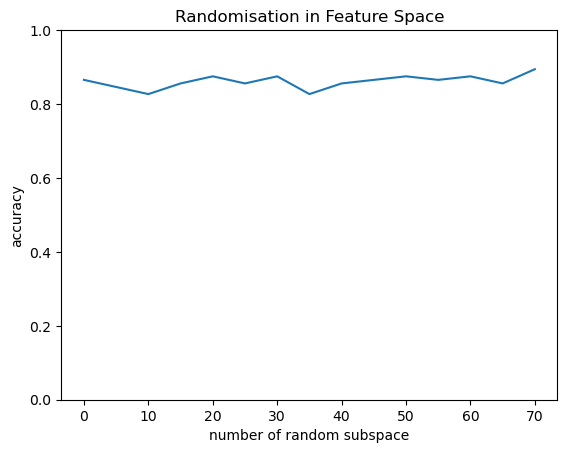
\includegraphics[width=\linewidth]{image/q3_fs_rs.png}
		\caption{Randomization in feature space}
		\label{fig:q3_fs}
	\end{subfigure}%
	\hfill
	\begin{subfigure}[t]{0.48\linewidth}
		\centering
		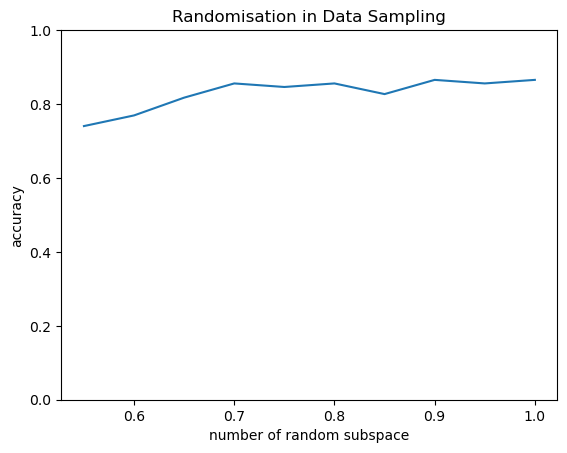
\includegraphics[width=\linewidth]{image/q3_data_rs.png}
		\caption{Random data subsamplint}
		\label{fig:q3_data}
	\end{subfigure}
	
	\begin{subfigure}[t]{0.48\linewidth}
		\centering
		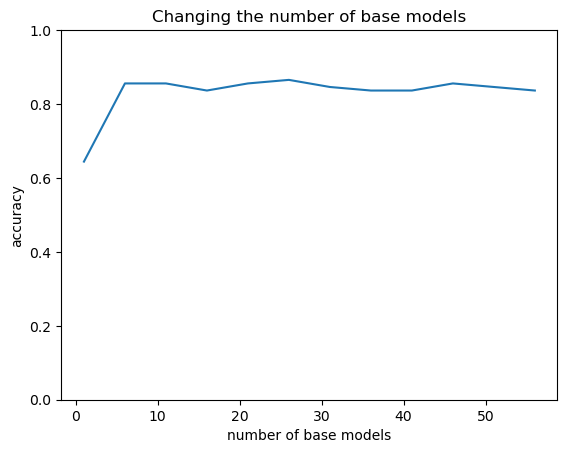
\includegraphics[width=\linewidth]{image/q3_basemodel.png}
		\caption{randomization in the number of basemodels}
		\label{fig:q3_base}
	\end{subfigure}
	\caption{Accuracy comparison between randomness parameters}
	\label{fig:q3_random}
\end{figure}

First, we look into randomization in feature space($M1$). As \cref{fig:q3_fs} indicates, the accuracy is almost highest when the number of random samples is around 30. This is because if the number of random vectors is too large, important features cannot be preserved, and if it is too small, overfitting occurs. Therefore, it is estimated that optimization occurred when the number of random vectors was 30.

Next, we observe the impact of data subsampling proportion($\alpha$). \cref{fig:q3_data} shows the accuracy with respect to the proportion of sub-sampled data. The more data we use, the better accuracy we get. This is quite predictable since the more data you have, the easier it is to generalize.

Lastly, regarding the effect of the number of base models($n_{model}$), we varied the number from 1 to 60, as shown in \cref{fig:q3_base}. When there are fewer than 30 models, the results are similar to a single PCA-LDA model. However, with more than 30 models, performance improves significantly, though further increases beyond 30 yield minimal gains. This is because up to 30 models, the ensemble can capture diverse features for generalization, but the PCA-LDA model’s limited ability to capture complex patterns prevents substantial improvement beyond that point. We used "majority voting" for combining predictions, as it’s most suitable for classification tasks where each class lacks numeric meaning, making it more appropriate than methods like averaging or maximum selection.

Considering both accuracy and computation cost, we conclude that the ensemble model with $M1=30$, $\alpha=0.9$, $n_{model}=30$ has the best performance.

% randomness parameter?

%-------------------------------------------------------------------------
\subsection{Result of PCA-LDA Ensemble}
The accuracy of committee machine, which gather all prediction results from each base models from ensemble model, is 0.846. And the average of individual models in ensemble model is 0.736. From this result, we can check that the performance of committee machine is better than individual as we learned. (Ensemble Learning LN, p.11-13)

In addition, \cref{fig:q3_2_cm} shows the confusion matrix of ensemble model. Compared to \cref{fig:q3_1_cm}, since \cref{fig:q3_2_cm} has less components outside the diagonal, we can visually check that the accuracy of classification of ensemble model is higher than single PCA-LDA model.

\section{Introduction}
\label{sec:intro}

Please follow the steps outlined below when submitting your manuscript to the IEEE Computer Society Press.
This style guide now has several important modifications (for example, you are no longer warned against the use of sticky tape to attach your artwork to the paper), so all authors should read this new version.

%-------------------------------------------------------------------------
\subsection{Language}

All manuscripts must be in English.

\subsection{Dual submission}

Please refer to the author guidelines on the \confName\ \confYear\ web page for a
discussion of the policy on dual submissions.

\subsection{Paper length}
Papers, excluding the references section, must be no longer than eight pages in length.
The references section will not be included in the page count, and there is no limit on the length of the references section.
For example, a paper of eight pages with two pages of references would have a total length of 10 pages.
{\bf There will be no extra page charges for \confName\ \confYear.}

Overlength papers will simply not be reviewed.
This includes papers where the margins and formatting are deemed to have been significantly altered from those laid down by this style guide.
Note that this \LaTeX\ guide already sets figure captions and references in a smaller font.
The reason such papers will not be reviewed is that there is no provision for supervised revisions of manuscripts.
The reviewing process cannot determine the suitability of the paper for presentation in eight pages if it is reviewed in eleven.

%-------------------------------------------------------------------------
\subsection{The ruler}
The \LaTeX\ style defines a printed ruler which should be present in the version submitted for review.
The ruler is provided in order that reviewers may comment on particular lines in the paper without circumlocution.
If you are preparing a document using a non-\LaTeX\ document preparation system, please arrange for an equivalent ruler to appear on the final output pages.
The presence or absence of the ruler should not change the appearance of any other content on the page.
The camera-ready copy should not contain a ruler.
(\LaTeX\ users may use options of \texttt{cvpr.sty} to switch between different versions.)

Reviewers:
note that the ruler measurements do not align well with lines in the paper --- this turns out to be very difficult to do well when the paper contains many figures and equations, and, when done, looks ugly.
Just use fractional references (\eg, this line is $087.5$), although in most cases one would expect that the approximate location will be adequate.


\subsection{Paper ID}
Make sure that the Paper ID from the submission system is visible in the version submitted for review (replacing the ``*****'' you see in this document).
If you are using the \LaTeX\ template, \textbf{make sure to update paper ID in the appropriate place in the tex file}.


\subsection{Mathematics}

Please number all of your sections and displayed equations as in these examples:
\begin{equation}
  E = m\cdot c^2
  \label{eq:important}
\end{equation}
and
\begin{equation}
  v = a\cdot t.
  \label{eq:also-important}
\end{equation}
It is important for readers to be able to refer to any particular equation.
Just because you did not refer to it in the text does not mean some future reader might not need to refer to it.
It is cumbersome to have to use circumlocutions like ``the equation second from the top of page 3 column 1''.
(Note that the ruler will not be present in the final copy, so is not an alternative to equation numbers).
All authors will benefit from reading Mermin's description of how to write mathematics:
\url{http://www.pamitc.org/documents/mermin.pdf}.

\subsection{Blind review}

Many authors misunderstand the concept of anonymizing for blind review.
Blind review does not mean that one must remove citations to one's own work---in fact it is often impossible to review a paper unless the previous citations are known and available.

Blind review means that you do not use the words ``my'' or ``our'' when citing previous work.
That is all.
(But see below for tech reports.)

Saying ``this builds on the work of Lucy Smith [1]'' does not say that you are Lucy Smith;
it says that you are building on her work.
If you are Smith and Jones, do not say ``as we show in [7]'', say ``as Smith and Jones show in [7]'' and at the end of the paper, include reference 7 as you would any other cited work.

An example of a bad paper just asking to be rejected:
\begin{quote}
\begin{center}
    An analysis of the frobnicatable foo filter.
\end{center}

   In this paper we present a performance analysis of our previous paper [1], and show it to be inferior to all previously known methods.
   Why the previous paper was accepted without this analysis is beyond me.

   [1] Removed for blind review
\end{quote}


An example of an acceptable paper:
\begin{quote}
\begin{center}
     An analysis of the frobnicatable foo filter.
\end{center}

   In this paper we present a performance analysis of the  paper of Smith \etal [1], and show it to be inferior to all previously known methods.
   Why the previous paper was accepted without this analysis is beyond me.

   [1] Smith, L and Jones, C. ``The frobnicatable foo filter, a fundamental contribution to human knowledge''. Nature 381(12), 1-213.
\end{quote}

If you are making a submission to another conference at the same time, which covers similar or overlapping material, you may need to refer to that submission in order to explain the differences, just as you would if you had previously published related work.
In such cases, include the anonymized parallel submission~\cite{Authors14} as supplemental material and cite it as
\begin{quote}
[1] Authors. ``The frobnicatable foo filter'', F\&G 2014 Submission ID 324, Supplied as supplemental material {\tt fg324.pdf}.
\end{quote}

Finally, you may feel you need to tell the reader that more details can be found elsewhere, and refer them to a technical report.
For conference submissions, the paper must stand on its own, and not {\em require} the reviewer to go to a tech report for further details.
Thus, you may say in the body of the paper ``further details may be found in~\cite{Authors14b}''.
Then submit the tech report as supplemental material.
Again, you may not assume the reviewers will read this material.

Sometimes your paper is about a problem which you tested using a tool that is widely known to be restricted to a single institution.
For example, let's say it's 1969, you have solved a key problem on the Apollo lander, and you believe that the 1970 audience would like to hear about your
solution.
The work is a development of your celebrated 1968 paper entitled ``Zero-g frobnication: How being the only people in the world with access to the Apollo lander source code makes us a wow at parties'', by Zeus \etal.

You can handle this paper like any other.
Do not write ``We show how to improve our previous work [Anonymous, 1968].
This time we tested the algorithm on a lunar lander [name of lander removed for blind review]''.
That would be silly, and would immediately identify the authors.
Instead write the following:
\begin{quotation}
\noindent
   We describe a system for zero-g frobnication.
   This system is new because it handles the following cases:
   A, B.  Previous systems [Zeus et al. 1968] did not  handle case B properly.
   Ours handles it by including a foo term in the bar integral.

   ...

   The proposed system was integrated with the Apollo lunar lander, and went all the way to the moon, don't you know.
   It displayed the following behaviours, which show how well we solved cases A and B: ...
\end{quotation}
As you can see, the above text follows standard scientific convention, reads better than the first version, and does not explicitly name you as the authors.
A reviewer might think it likely that the new paper was written by Zeus \etal, but cannot make any decision based on that guess.
He or she would have to be sure that no other authors could have been contracted to solve problem B.
\medskip

\noindent
FAQ\medskip\\
{\bf Q:} Are acknowledgements OK?\\
{\bf A:} No.  Leave them for the final copy.\medskip\\
{\bf Q:} How do I cite my results reported in open challenges?
{\bf A:} To conform with the double-blind review policy, you can report results of other challenge participants together with your results in your paper.
For your results, however, you should not identify yourself and should not mention your participation in the challenge.
Instead present your results referring to the method proposed in your paper and draw conclusions based on the experimental comparison to other results.\medskip\\

\begin{figure}[t]
  \centering
  \fbox{\rule{0pt}{2in} \rule{0.9\linewidth}{0pt}}
   %\includegraphics[width=0.8\linewidth]{egfigure.eps}

   \caption{Example of caption.
   It is set in Roman so that mathematics (always set in Roman: $B \sin A = A \sin B$) may be included without an ugly clash.}
   \label{fig:onecol}
\end{figure}

\subsection{Miscellaneous}

\noindent
Compare the following:\\
\begin{tabular}{ll}
 \verb'$conf_a$' &  $conf_a$ \\
 \verb'$\mathit{conf}_a$' & $\mathit{conf}_a$
\end{tabular}\\
See The \TeX book, p165.

The space after \eg, meaning ``for example'', should not be a sentence-ending space.
So \eg is correct, {\em e.g.} is not.
The provided \verb'\eg' macro takes care of this.

When citing a multi-author paper, you may save space by using ``et alia'', shortened to ``\etal'' (not ``{\em et.\ al.}'' as ``{\em et}'' is a complete word).
If you use the \verb'\etal' macro provided, then you need not worry about double periods when used at the end of a sentence as in Alpher \etal.
However, use it only when there are three or more authors.
Thus, the following is correct:
   ``Frobnication has been trendy lately.
   It was introduced by Alpher~\cite{Alpher02}, and subsequently developed by
   Alpher and Fotheringham-Smythe~\cite{Alpher03}, and Alpher \etal~\cite{Alpher04}.''

This is incorrect: ``... subsequently developed by Alpher \etal~\cite{Alpher03} ...'' because reference~\cite{Alpher03} has just two authors.

\begin{figure*}
  \centering
  \begin{subfigure}{0.68\linewidth}
    \fbox{\rule{0pt}{2in} \rule{.9\linewidth}{0pt}}
    \caption{An example of a subfigure.}
    \label{fig:short-a}
  \end{subfigure}
  \hfill
  \begin{subfigure}{0.28\linewidth}
    \fbox{\rule{0pt}{2in} \rule{.9\linewidth}{0pt}}
    \caption{Another example of a subfigure.}
    \label{fig:short-b}
  \end{subfigure}
  \caption{Example of a short caption, which should be centered.}
  \label{fig:short}
\end{figure*}

\section{Formatting your paper}
\label{sec:formatting}

All text must be in a two-column format.
The total allowable size of the text area is $6\frac78$ inches (17.46 cm) wide by $8\frac78$ inches (22.54 cm) high.
Columns are to be $3\frac14$ inches (8.25 cm) wide, with a $\frac{5}{16}$ inch (0.8 cm) space between them.
The main title (on the first page) should begin 1 inch (2.54 cm) from the top edge of the page.
The second and following pages should begin 1 inch (2.54 cm) from the top edge.
On all pages, the bottom margin should be $1\frac{1}{8}$ inches (2.86 cm) from the bottom edge of the page for $8.5 \times 11$-inch paper;
for A4 paper, approximately $1\frac{5}{8}$ inches (4.13 cm) from the bottom edge of the
page.

%-------------------------------------------------------------------------
\subsection{Margins and page numbering}

All printed material, including text, illustrations, and charts, must be kept
within a print area $6\frac{7}{8}$ inches (17.46 cm) wide by $8\frac{7}{8}$ inches (22.54 cm)
high.
%
Page numbers should be in the footer, centered and $\frac{3}{4}$ inches from the bottom of the page.
The review version should have page numbers, yet the final version submitted as camera ready should not show any page numbers.
The \LaTeX\ template takes care of this when used properly.



%-------------------------------------------------------------------------
\subsection{Type style and fonts}

Wherever Times is specified, Times Roman may also be used.
If neither is available on your word processor, please use the font closest in
appearance to Times to which you have access.

MAIN TITLE.
Center the title $1\frac{3}{8}$ inches (3.49 cm) from the top edge of the first page.
The title should be in Times 14-point, boldface type.
Capitalize the first letter of nouns, pronouns, verbs, adjectives, and adverbs;
do not capitalize articles, coordinate conjunctions, or prepositions (unless the title begins with such a word).
Leave two blank lines after the title.

AUTHOR NAME(s) and AFFILIATION(s) are to be centered beneath the title
and printed in Times 12-point, non-boldface type.
This information is to be followed by two blank lines.

The ABSTRACT and MAIN TEXT are to be in a two-column format.

MAIN TEXT.
Type main text in 10-point Times, single-spaced.
Do NOT use double-spacing.
All paragraphs should be indented 1 pica (approx.~$\frac{1}{6}$ inch or 0.422 cm).
Make sure your text is fully justified---that is, flush left and flush right.
Please do not place any additional blank lines between paragraphs.

Figure and table captions should be 9-point Roman type as in \cref{fig:onecol,fig:short}.
Short captions should be centred.

\noindent Callouts should be 9-point Helvetica, non-boldface type.
Initially capitalize only the first word of section titles and first-, second-, and third-order headings.

FIRST-ORDER HEADINGS.
(For example, {\large \bf 1. Introduction}) should be Times 12-point boldface, initially capitalized, flush left, with one blank line before, and one blank line after.

SECOND-ORDER HEADINGS.
(For example, { \bf 1.1. Database elements}) should be Times 11-point boldface, initially capitalized, flush left, with one blank line before, and one after.
If you require a third-order heading (we discourage it), use 10-point Times, boldface, initially capitalized, flush left, preceded by one blank line, followed by a period and your text on the same line.

%-------------------------------------------------------------------------
\subsection{Footnotes}

Please use footnotes\footnote{This is what a footnote looks like.
It often distracts the reader from the main flow of the argument.} sparingly.
Indeed, try to avoid footnotes altogether and include necessary peripheral observations in the text (within parentheses, if you prefer, as in this sentence).
If you wish to use a footnote, place it at the bottom of the column on the page on which it is referenced.
Use Times 8-point type, single-spaced.


%-------------------------------------------------------------------------
\subsection{Cross-references}

For the benefit of author(s) and readers, please use the
{\small\begin{verbatim}
  \cref{...}
\end{verbatim}}  command for cross-referencing to figures, tables, equations, or sections.
This will automatically insert the appropriate label alongside the cross-reference as in this example:
\begin{quotation}
  To see how our method outperforms previous work, please see \cref{fig:onecol} and \cref{tab:example}.
  It is also possible to refer to multiple targets as once, \eg~to \cref{fig:onecol,fig:short-a}.
  You may also return to \cref{sec:formatting} or look at \cref{eq:also-important}.
\end{quotation}
If you do not wish to abbreviate the label, for example at the beginning of the sentence, you can use the
{\small\begin{verbatim}
  \Cref{...}
\end{verbatim}}
command. Here is an example:
\begin{quotation}
  \Cref{fig:onecol} is also quite important.
\end{quotation}

%-------------------------------------------------------------------------
\subsection{References}

List and number all bibliographical references in 9-point Times, single-spaced, at the end of your paper.
When referenced in the text, enclose the citation number in square brackets, for
example~\cite{Authors14}.
Where appropriate, include page numbers and the name(s) of editors of referenced books.
When you cite multiple papers at once, please make sure that you cite them in numerical order like this \cite{Alpher02,Alpher03,Alpher05,Authors14b,Authors14}.
If you use the template as advised, this will be taken care of automatically.

\begin{table}
  \centering
  \begin{tabular}{@{}lc@{}}
    \toprule
    Method & Frobnability \\
    \midrule
    Theirs & Frumpy \\
    Yours & Frobbly \\
    Ours & Makes one's heart Frob\\
    \bottomrule
  \end{tabular}
  \caption{Results.   Ours is better.}
  \label{tab:example}
\end{table}

%-------------------------------------------------------------------------
\subsection{Illustrations, graphs, and photographs}

All graphics should be centered.
In \LaTeX, avoid using the \texttt{center} environment for this purpose, as this adds potentially unwanted whitespace.
Instead use
{\small\begin{verbatim}
  \centering
\end{verbatim}}
at the beginning of your figure.
Please ensure that any point you wish to make is resolvable in a printed copy of the paper.
Resize fonts in figures to match the font in the body text, and choose line widths that render effectively in print.
Readers (and reviewers), even of an electronic copy, may choose to print your paper in order to read it.
You cannot insist that they do otherwise, and therefore must not assume that they can zoom in to see tiny details on a graphic.

When placing figures in \LaTeX, it's almost always best to use \verb+\includegraphics+, and to specify the figure width as a multiple of the line width as in the example below
{\small\begin{verbatim}
   \usepackage{graphicx} ...
   \includegraphics[width=0.8\linewidth]
                   {myfile.pdf}
\end{verbatim}
}


%-------------------------------------------------------------------------
\subsection{Color}

Please refer to the author guidelines on the \confName\ \confYear\ web page for a discussion of the use of color in your document.

If you use color in your plots, please keep in mind that a significant subset of reviewers and readers may have a color vision deficiency; red-green blindness is the most frequent kind.
Hence avoid relying only on color as the discriminative feature in plots (such as red \vs green lines), but add a second discriminative feature to ease disambiguation.
\section{Final copy}

You must include your signed IEEE copyright release form when you submit your finished paper.
We MUST have this form before your paper can be published in the proceedings.

Please direct any questions to the production editor in charge of these proceedings at the IEEE Computer Society Press:
\url{https://www.computer.org/about/contact}.
{
    \small
    \bibliographystyle{ieeenat_fullname}
    \bibliography{main}
}

% WARNING: do not forget to delete the supplementary pages from your submission 
% \clearpage
\setcounter{page}{1}
\maketitlesupplementary


\section{Rationale}
\label{sec:rationale}
% 
Having the supplementary compiled together with the main paper means that:
% 
\begin{itemize}
\item The supplementary can back-reference sections of the main paper, for example, we can refer to \cref{sec:intro};
\item The main paper can forward reference sub-sections within the supplementary explicitly (e.g. referring to a particular experiment); 
\item When submitted to arXiv, the supplementary will already included at the end of the paper.
\end{itemize}
% 
To split the supplementary pages from the main paper, you can use \href{https://support.apple.com/en-ca/guide/preview/prvw11793/mac#:~:text=Delete%20a%20page%20from%20a,or%20choose%20Edit%20%3E%20Delete).}{Preview (on macOS)}, \href{https://www.adobe.com/acrobat/how-to/delete-pages-from-pdf.html#:~:text=Choose%20%E2%80%9CTools%E2%80%9D%20%3E%20%E2%80%9COrganize,or%20pages%20from%20the%20file.}{Adobe Acrobat} (on all OSs), as well as \href{https://superuser.com/questions/517986/is-it-possible-to-delete-some-pages-of-a-pdf-document}{command line tools}.

\end{document}
